\subsection{Beugung}
Dieser Versuch befasst sich mit der Beugung von Strahlen. Sobald eine sich geradlinig fortbewegende Welle abweicht ist die Rede von Beugung. Beugung tritt überall dort ein wo eine Welle durch ein Hinderniss begrenzt wird, so dass sich die Welle um das Hinderniss ''herumbeugen'' muss.

\subsection{Interferenz}

Befinden sich mehrere Hindernisse in der Laufrichtung der Welle, wie z.B bei einem Spalt (je Kannte ein Hinderniss) oder bei einem Doppelspalt (Abb. \ref{fig:wellen}), so enstehen zwei Beugungen. Vorausgesetz die Wellenlänge $\lambda$ und der Phasenwinkel $\phi$ der Lichtquelle ist bei beiden Lichtquellen der Selbe so interverieren die Lichtquellen miteinander \cite{FHNWBEUGUNG}.
%%%%%%%%%%%%%%%%%%%%%%%%%%%%%%%%%%%%%%%%%%%%%%%%%%%%%%%%%%%%%%%%%%%%%%%%%%%%%
\begin{figure}[htb]
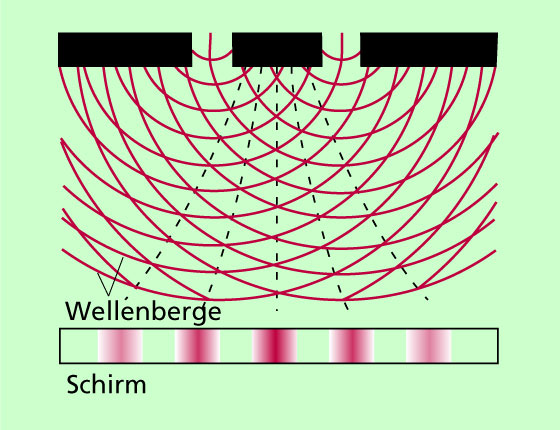
\includegraphics[width=\textwidth]{wellen_berge.jpg}
\caption{Interferenz am Doppelspalt \cite{LERN}} % picture caption
\label{fig:wellen}
\end{figure}
%%%%%%%%%%%%%%%%%%%%%%%%%%%%%%%%%%%%%%%%%%%%%%%%%%%%%%%%%%%%%%%%%%%%%%%%%%%%%
Das Interferenzmuster lässt sich leicht mittels eines Schirmes visualisiern. Der Schirm sollte dazu nicht alzu nahe an den Hindernissen Befinden. Auf dem Schirm können nun die Maxima und Minima der interferierenden Wellen beobachtet werden.

\newpage
\subsection{Frauenhofer'sche Beobachtungsart}

Bei diesem Versuch wird die Frauenhofer'sche Beobachtungsart untersucht. Dabei wird, wie in der Abbildung \ref{fig:Frauenhofer} erkennbar, mit hilfe einer Linse das Interferenzmuster auf ein Schirm projeziert. Zu diesem Zweck muss sich die Linse im Abstand deren Brennweite $f$ vor dem Schirm platziert werden. Dies ermöglicht die betrachtung des Interferenzmusters in einm grossen Abstand zu Quelle. Das beobachtete Muster unterscheidet sich lediglich durch einen Skalierungsfaktor.
%%%%%%%%%%%%%%%%%%%%%%%%%%%%%%%%%%%%%%%%%%%%%%%%%%%%%%%%%%%%%%%%%%%%%%%%%%%%%
\begin{figure}[htb]
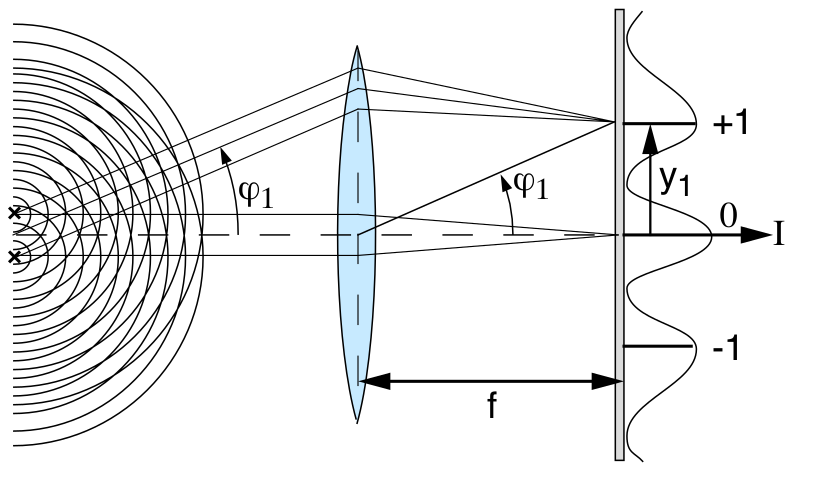
\includegraphics[width=\textwidth]{frauen_beugung.png}
\caption{Frauenhofer'sche Beobachtungsart \cite{FHNWO9}} % picture caption
\label{fig:Frauenhofer}
\end{figure}
%%%%%%%%%%%%%%%%%%%%%%%%%%%%%%%%%%%%%%%%%%%%%%%%%%%%%%%%%%%%%%%%%%%%%%%%%%%%%
\newline
Die in der Abbildung \ref{fig:Frauenhofer} eingezeichneten Grössen hängen wie folgt zusammen:\\

%%%%%%%%%%%%%%%%%%%%%%%%%%%%%%%%%%%%%%%%%%%%%%%%%%%%%%%%%%%%%%%%%%%%%%%%%%%%%
\begin{equation}
tan({\phi}_{1}) = \frac{y_1}{f}
\label{eq:frauen}
\end{equation}
%%%%%%%%%%%%%%%%%%%%%%%%%%%%%%%%%%%%%%%%%%%%%%%%%%%%%%%%%%%%%%%%%%%%%%%%%%%%%
